\chapter{評価}
Stuguinシステムが,ユーザが抱く動機づけタイプに応じてアプローチを切り替えることにより,学習に対する動機づけを向上及び内在化させることができたかどうか評価する.
本章ではまず評価概要を説明し,実験結果を示す.最後に,評価実験から得られた結果をもとに考察を行う.

\section{評価実験の概要}
本瀬越では,本研究における評価実験の概要を述べる.はじめに,評価実験を行う目的を説明する.
ついで,評価実験を行う手順について説明する.

\subsection{評価の目的}
本研究では,学習者が抱く動機づけタイプに応じたアプローチが,動機づけの向上及び内在化に貢献するかを評価する.
前述したように,動機づけはその自己決定度合いに基づいて無調整,外的調整,取り入れ的調整,同一化的調整,統合的調整,内的調整の6種類に分類でき,各タイプごとに特徴や動機づけが生じる要因が存在する~\cite{ryan2000self}.
これらの動機づけは,内的であるほど満足感が高く,より持続するとされている.
基本的には,外的な動機づけ要因は動機づけの内在化を妨げるものの~\cite{moller2006self}~\cite{shimizu},たとえ外発的に動機づけられた学習であっても,その学習に対する個人の価値の認め方によっては,自己決定性は高くなる.
つまり,学習者抱く動機づけに応じたアプローチを行うことが,動機づけの向上及び内在化に繋がると考えられる.
したがって本研究では,動機づけタイプに応じたアプローチが動機づけの向上及び内在化に有用な方策であるかを評価することを目的とする.

\subsection{評価実験手法}
今回の評価実験では,慶應義塾大学のドイツ語履修者10名,英語履修者5名の計15名を対象に実験を行なった.
被験者は自身が保有しているiPhoneにStuguinをインストールし,ドイツ語履修者はドイツ語の学習記録管理として,英語履修者は英語の学習記録管理として,任意のタイミングで使用してもらった.
1週間に一度,学習に対する動機づけタイプを測定するアンケートに回答してもらい,内在化アプローチモジュールにて表示する機能を選定した.
この被験者15名を表~\ref{tb:group}のように3群に分け,それぞれで内在化アプローチモジュールの挙動を変えた.

\begin{table}[htb]
\begin{center}
  \begin{tabular}{|l|l|l|} \hline
    グループ & 挙動 & 人数 \\ \hline
	{\bf Same}群 & トップ画面に自身の動機づけタイプに適した機能が表示される & 5名 \\
    {\bf Wrong}群 & トップ画面に自身の動機づけタイプに適した機能とは異なる機能が表示される & 5名 \\
    {\bf None}群 & トップ画面に機能が表示されない & 5名 \\ \hline
  \end{tabular}
  \caption{被験者グループ}
  \label{tb:group}
\end{center}
\end{table}

{\bf Same}群はモジュールの挙動通り,ユーザが抱く動機づけタイプに適した機能が表示される.
外的調整の場合はポイント機能,取り入れ的調整の場合はランキング機能,同一化的調整の場合は目標設定機能が表示され,内的調整の場合はどの機能も表示されない.
対して{\bf Wrong}群は,ユーザが抱く動機づけタイプに適した機能とは異なる機能が表示される.
外的調整の場合はランキング機能か目標設定機能のどちらか,取り入れ的調整の場合はポイント機能か目標設定機能のどちらか,同一化的調整の場合はポイント機能かランキング機能のどちらか,内的機能は全ての機能から1つ,ランダムに表示される.
なお,どちらの群においても,1週間同じ機能が表示される.
コントロールグループである{\bf None}群は,実験期間中どの機能も表示されない.
{\bf None}群のトップ画面は図~\ref{fig:none_group}のようになる.

\begin{figure}[hb]
	\begin{center}
	\fbox{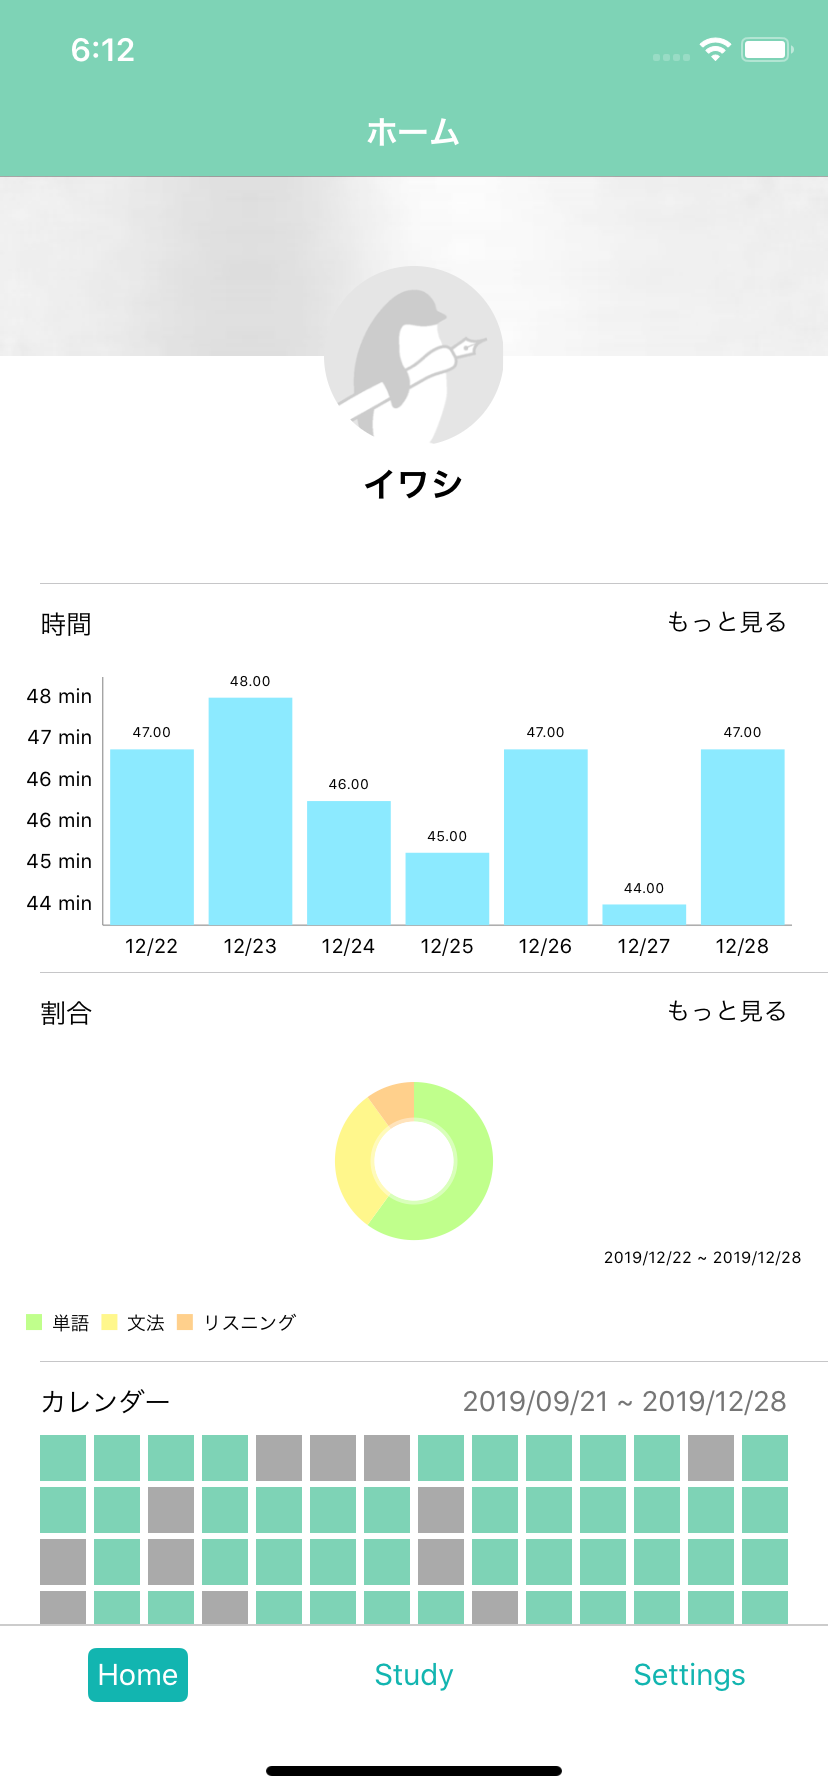
\includegraphics[width=5cm]{images/7/none_group.png}}
	\caption{None群のトップ画面}
	\label{fig:none_group}
	\end{center}
\end{figure}

本研究では動機づけタイプに応じてアプローチを切り替える手法が学習に対する動機づけに与える影響を見ることを目的としているため,被験者の学習時間,学習頻度,システムの利用頻度及びアンケートにより判定される動機づけの変容について評価する.

\section{評価結果}
本節では,動機づけタイプに応じてアプローチを切り替える手法が学習に対する動機づけに与える影響について,本評価実験で得られた評価結果を示す.
図~\ref{tb:same_motivation_type}, ~\ref{tb:wrong_motivation_type}, ~\ref{tb:none_motivation_type}の表にアンケートから判定した各群の動機づけタイプの遷移を示す.
多少の変動はあるが,どの群においても動機づけタイプが変化したと言える被験者は存在しなかった.

\begin{figure}[htb]
\begin{center}
\begin{tabular}{c}

  \begin{minipage}[htb]{\linewidth}
  \begin{center}
  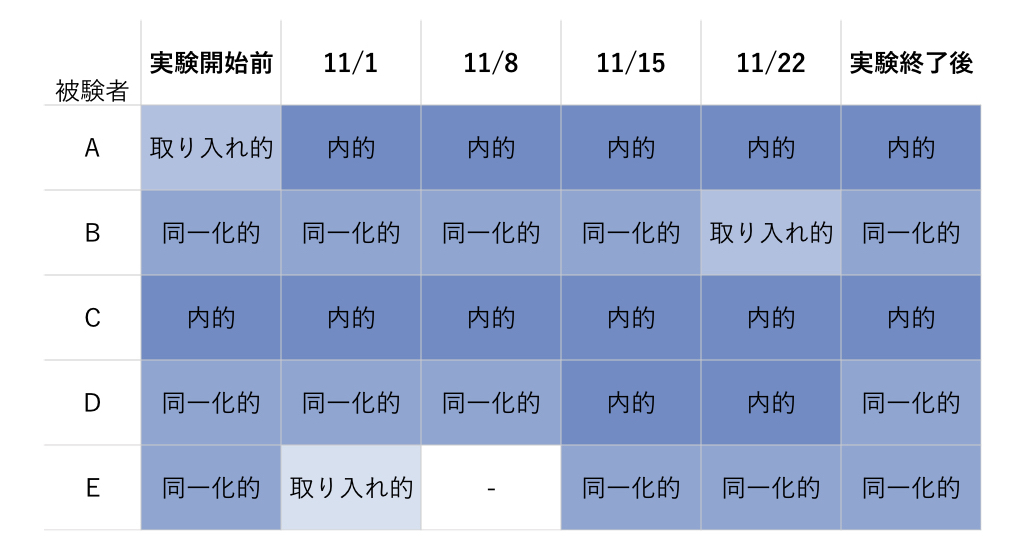
\includegraphics[width=12cm]{images/7/same_motivation_type.png}
  \caption{Same群の動機づけタイプの遷移}
  \label{tb:same_motivation_type}
  \end{center}
  \end{minipage}

  \\

  \begin{minipage}[htb]{\linewidth}
  \begin{center}
  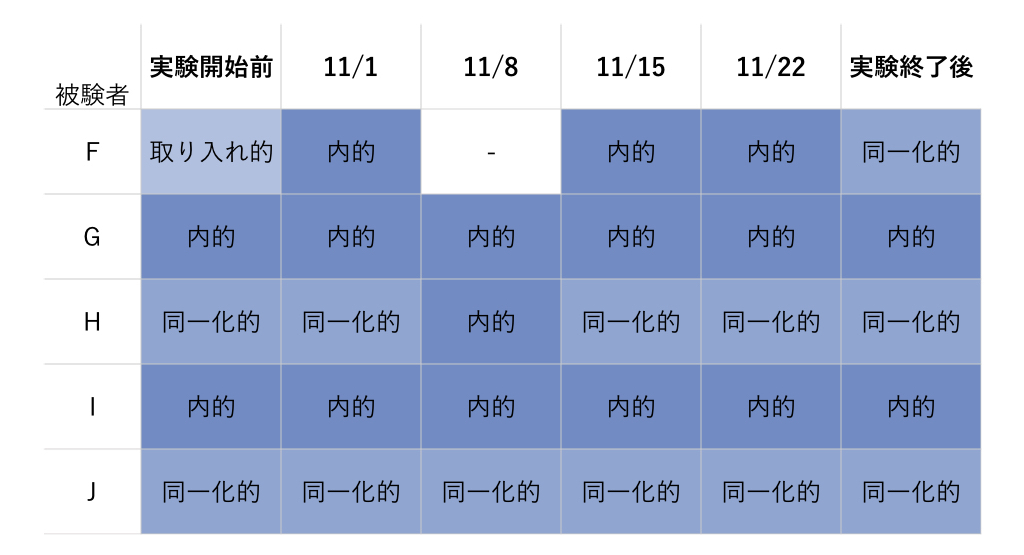
\includegraphics[width=12cm]{images/7/wrong_motivation_type.png}
  \caption{Wrong群の動機づけタイプの遷移}
  \label{tb:wrong_motivation_type}
  \end{center}
  \end{minipage}

  \\

  \begin{minipage}[htb]{\linewidth}
  \begin{center}
  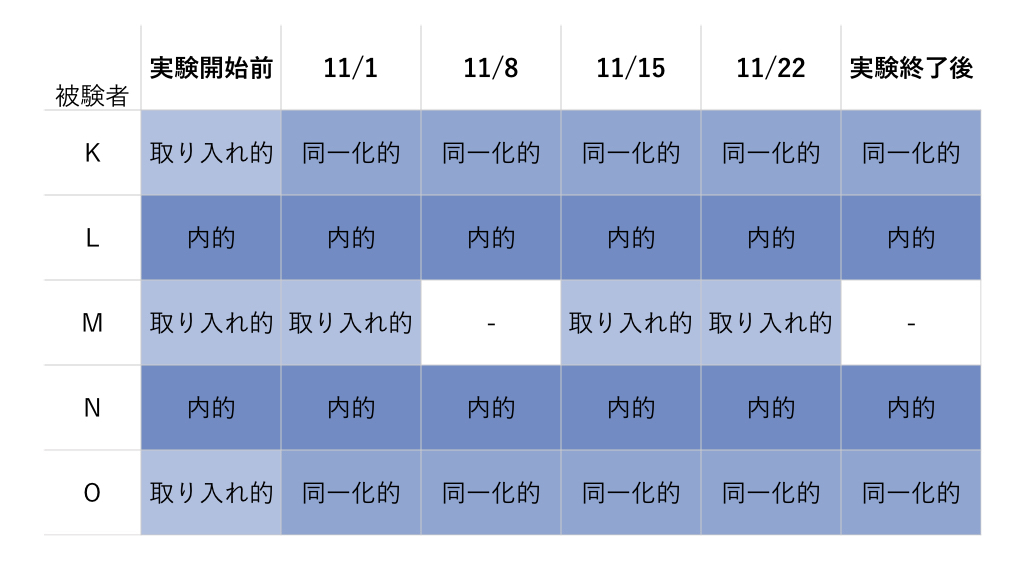
\includegraphics[width=12cm]{images/7/none_motivation_type.png}
  \caption{None群の動機づけタイプの遷移}
  \label{tb:none_motivation_type}
  \end{center}
  \end{minipage}

\end{tabular}
\end{center}
\end{figure}

図~\ref{fig:total_study_time}に各群の実験期間中における総学習時間を,図~\ref{fig:total_study_count}に各群の実験期間中における総学習記録回数を,図~\ref{fig:app_open_count}に各群の実験期間中におけるアプリケーションの総起動回数を示す.
Wrong群は総学習時間が最も短く,総学習記録回数が最も多い結果となった.

\begin{figure}[htb]
\begin{center}
\begin{tabular}{c}

\begin{minipage}[htb]{\linewidth}
  \begin{center}
  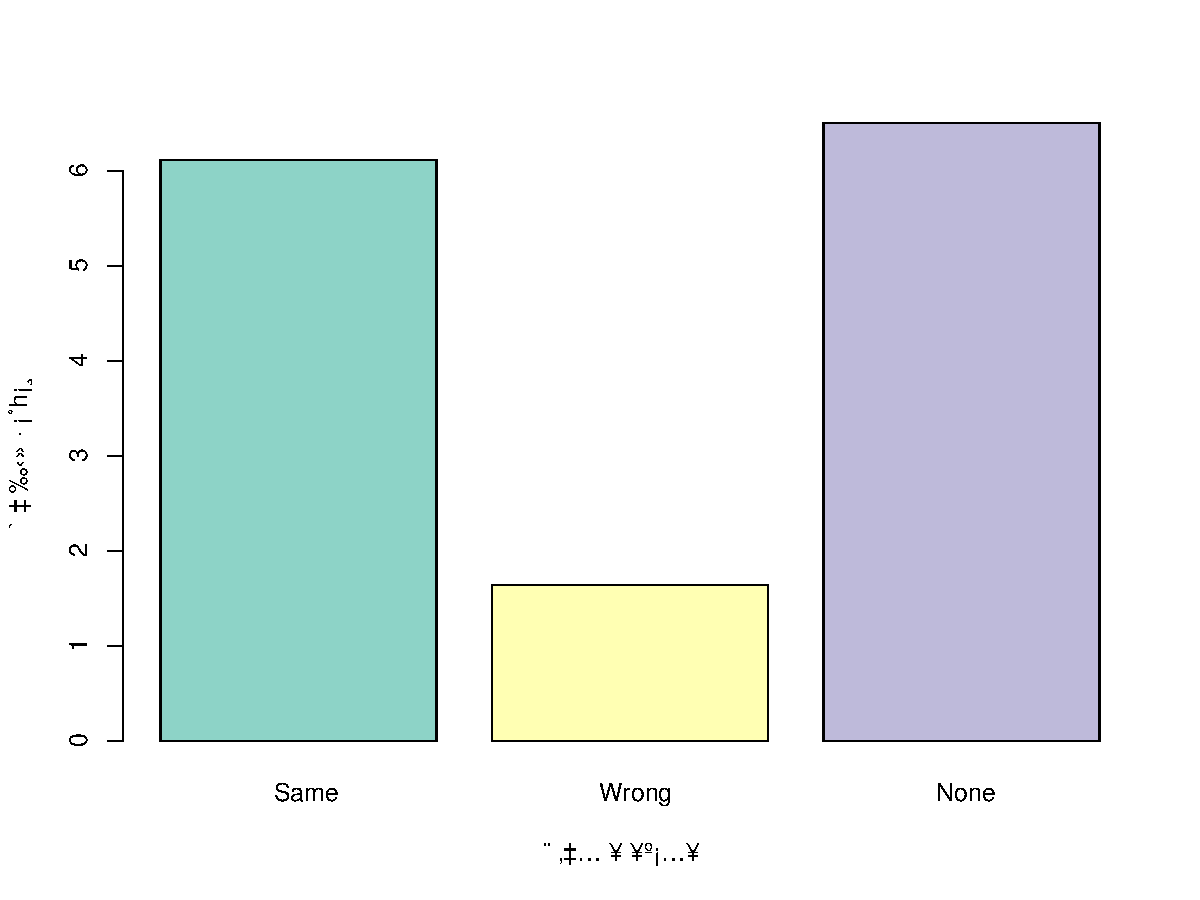
\includegraphics[width=9cm]{images/7/total_study_time.pdf}
  \caption{実験期間中の総学習時間}
  \label{fig:total_study_time}
  \end{center}
\end{minipage}

\\

\begin{minipage}[htb]{\linewidth}
  \begin{center}
  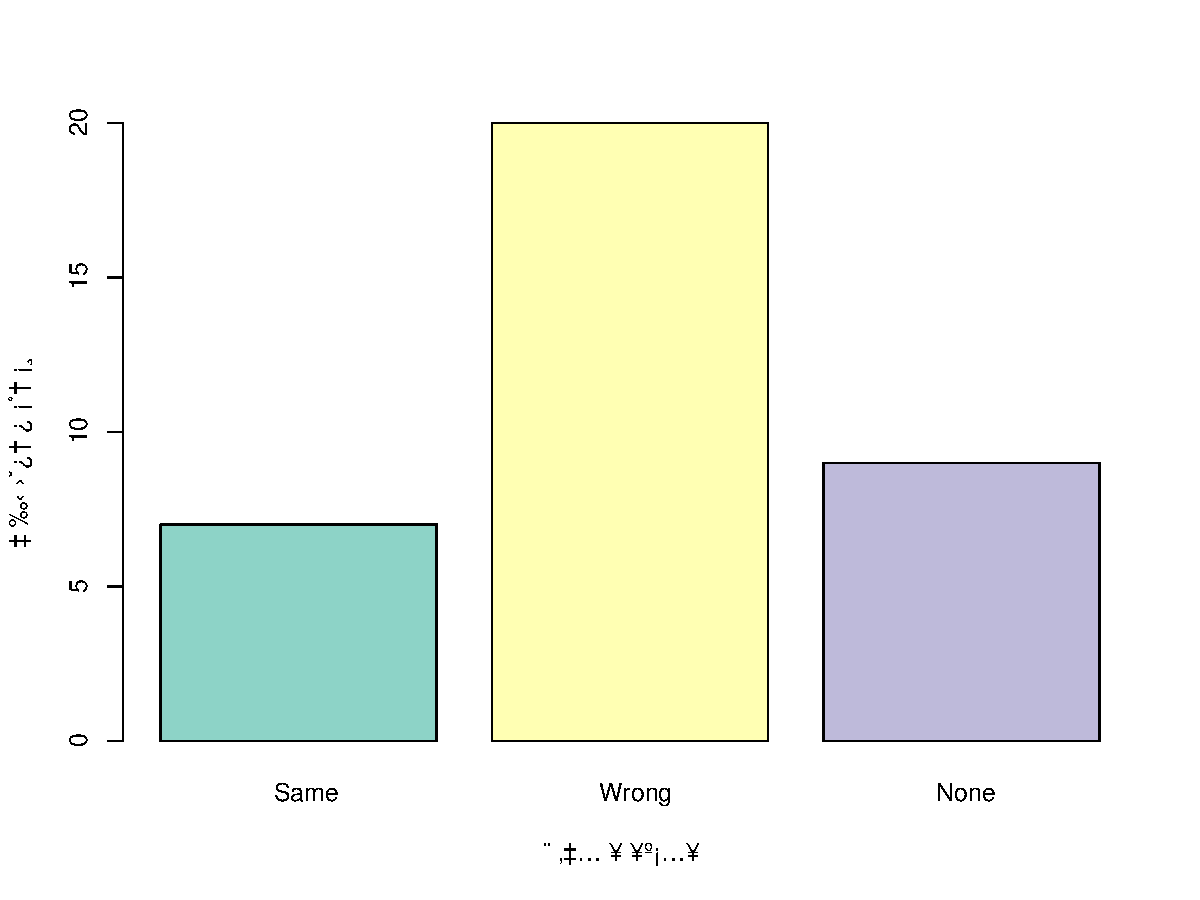
\includegraphics[width=9cm]{images/7/total_study_count.pdf}
  \caption{実験期間中の総学習記録回数}
  \label{fig:total_study_count}
  \end{center}
\end{minipage}

\\

\begin{minipage}[htb]{\linewidth}
  \begin{center}
  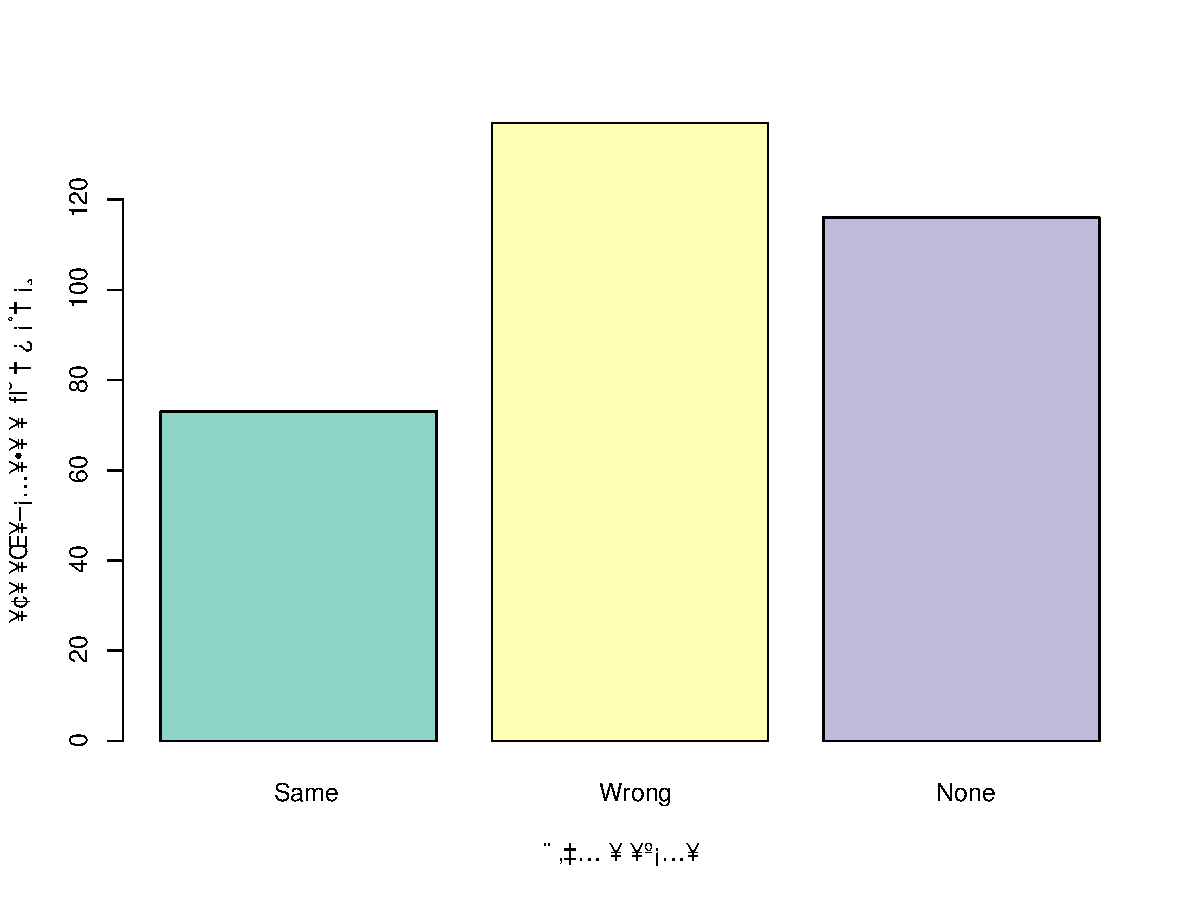
\includegraphics[width=9cm]{images/7/app_open_count.pdf}
  \caption{実験期間中のアプリケーション総起動回数}
  \label{fig:app_open_count}
  \end{center}
\end{minipage}

\end{tabular}
\end{center}
\end{figure}

図~\ref{fig:same_records_ratio}, ~\ref{fig:wrong_records_ratio}, ~\ref{fig:none_records_ratio}に各群における学習記録の内訳を示す.
Wrong群の被験者が記録した学習記録のほとんどが,実際に計測されたものであった.

\begin{figure}[htb]
\begin{center}
\begin{tabular}{c}

  \begin{minipage}[htb]{0.5\linewidth}
  \begin{center}
  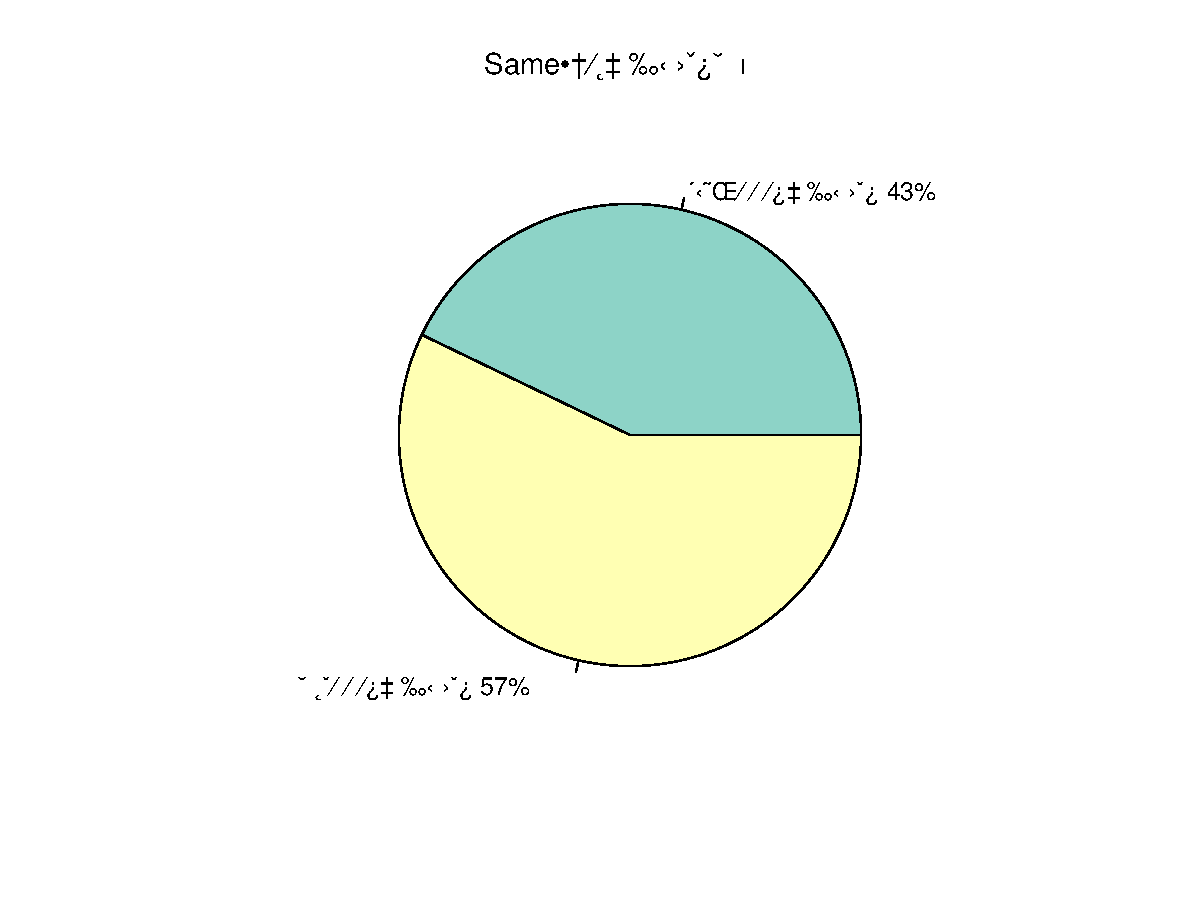
\includegraphics[width=9cm]{images/7/same_records_ratio.pdf}
  \caption{Same群の学習記録内訳}
  \label{fig:same_records_ratio}
  \end{center}
  \end{minipage}

  \begin{minipage}[htb]{0.5\linewidth}
  \begin{center}
  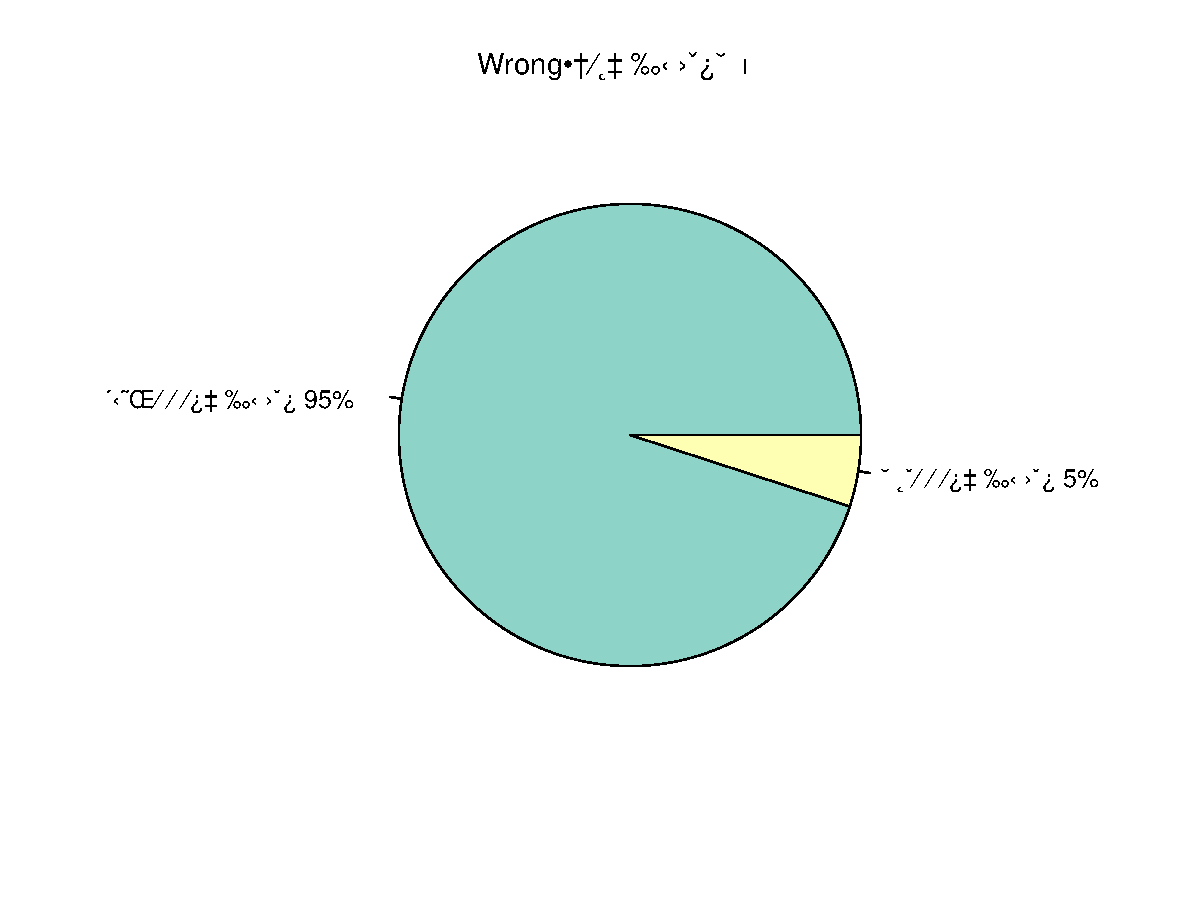
\includegraphics[width=9cm]{images/7/wrong_records_ratio.pdf}
  \caption{Wrong群の学習記録内訳}
  \label{fig:wrong_records_ratio}
  \end{center}
  \end{minipage}

  \\

  \begin{minipage}[htb]{\linewidth}
  \begin{center}
  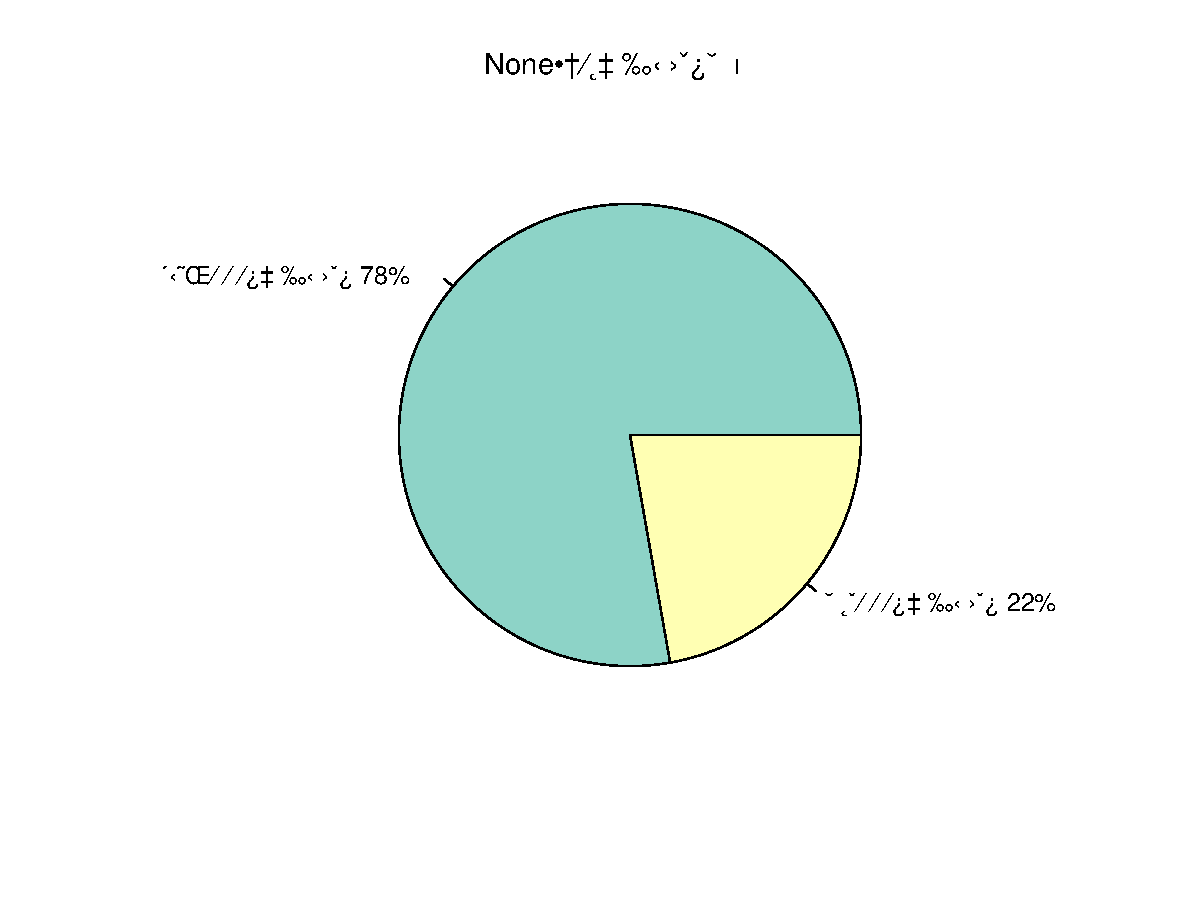
\includegraphics[width=9cm]{images/7/none_records_ratio.pdf}
  \caption{None群の学習記録内訳}
  \label{fig:none_records_ratio}
  \end{center}
  \end{minipage}

\end{tabular}
\end{center}
\end{figure}

また図~\ref{fig:same_feature}にSame群の被験者に表示された機能を,~\ref{fig:wrong_feature}にWrong群の被験者に表示された機能を示す.

\begin{figure}[h]
  \begin{center}
  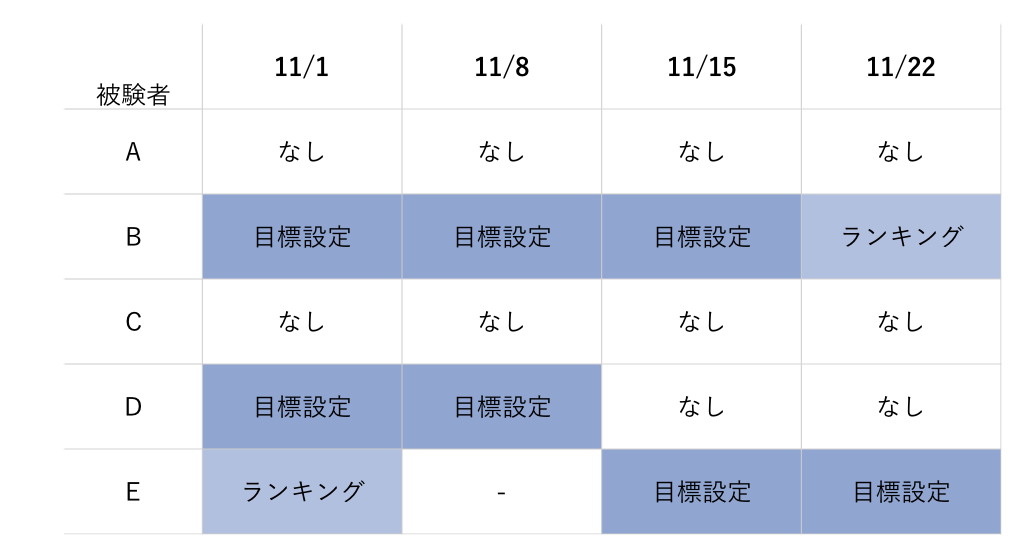
\includegraphics[width=12cm]{images/7/same_feature.png}
  \caption{Same群の被験者に表示された機能}
  \label{fig:same_feature}
  \end{center}
\end{figure}

\begin{figure}[h]
  \begin{center}
  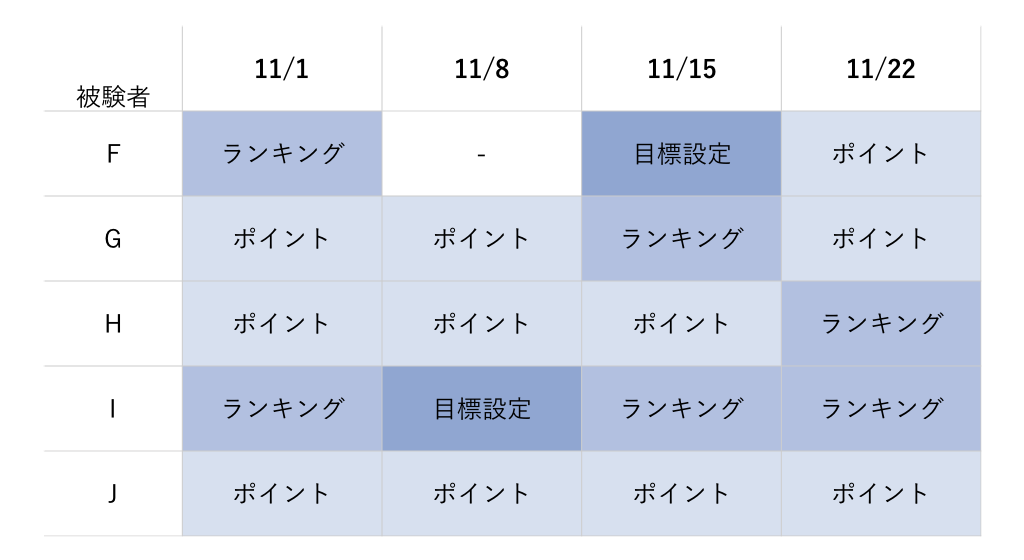
\includegraphics[width=12cm]{images/7/wrong_feature.png}
  \caption{Wrong群の被験者に表示された機能}
  \label{fig:wrong_feature}
  \end{center}
\end{figure}

図~\ref{fig:same_study_count}, ~\ref{fig:wrong_study_count}, ~\ref{fig:none_study_count}に各群の被験者の学習記録回数の遷移を示す.
どの群においても実験期間後半はほとんど学習が記録されなかった.

\begin{figure}[htb]
\begin{center}
\begin{tabular}{c}

  \begin{minipage}[htb]{\linewidth}
  \begin{center}
  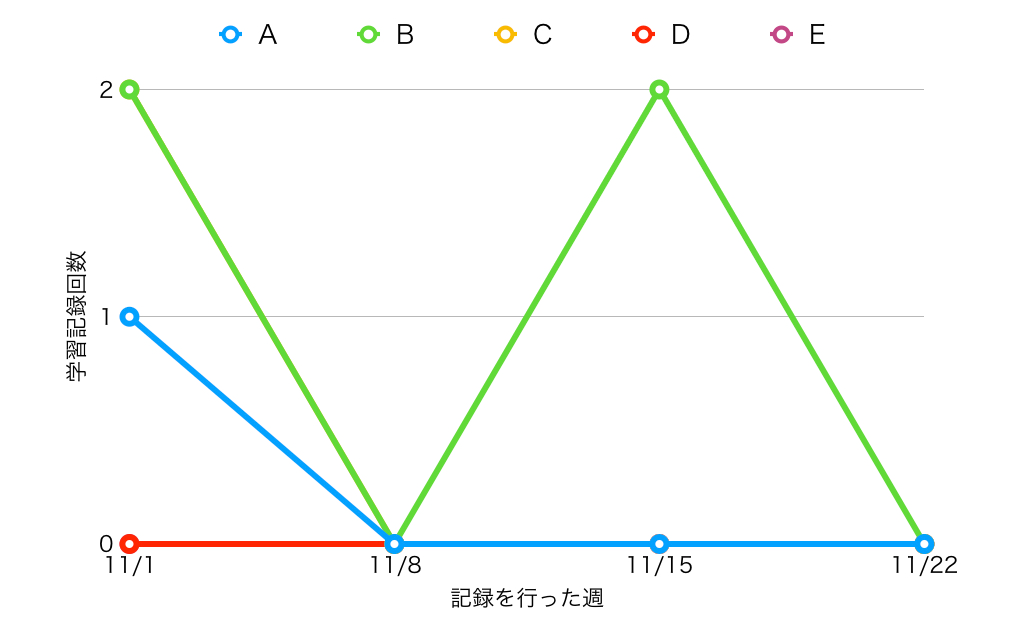
\includegraphics[width=10cm]{images/7/same_study_count.png}
  \caption{Same群の学習記録回数の遷移}
  \label{fig:same_study_count}
  \end{center}
  \end{minipage}

  \\

  \begin{minipage}[htb]{\linewidth}
  \begin{center}
  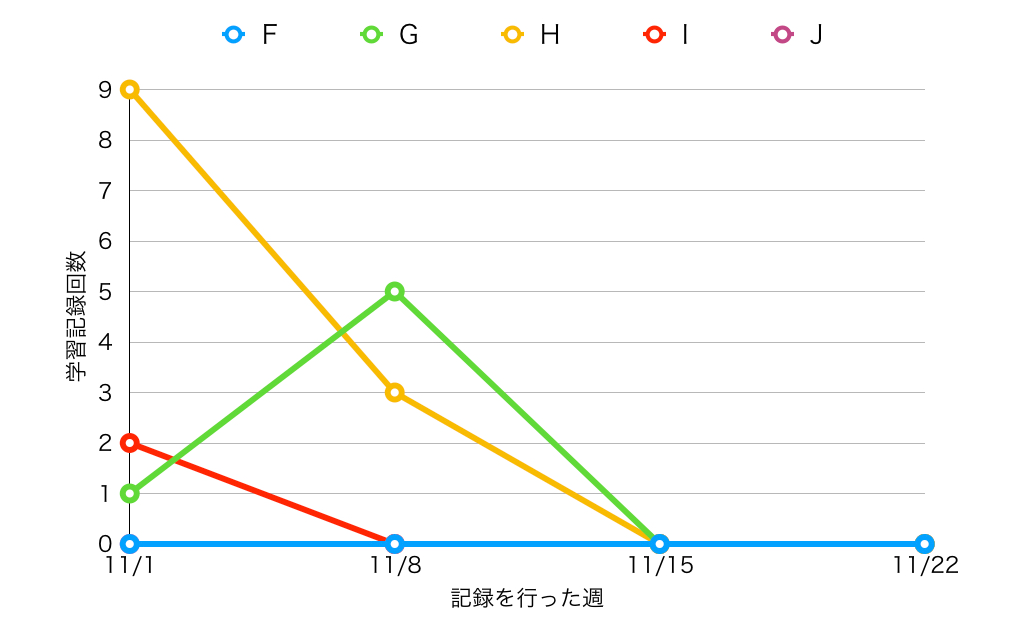
\includegraphics[width=10cm]{images/7/wrong_study_count.png}
  \caption{Wrong群の学習記録回数の遷移}
  \label{fig:wrong_study_count}
  \end{center}
  \end{minipage}

  \\

  \begin{minipage}[htb]{\linewidth}
  \begin{center}
  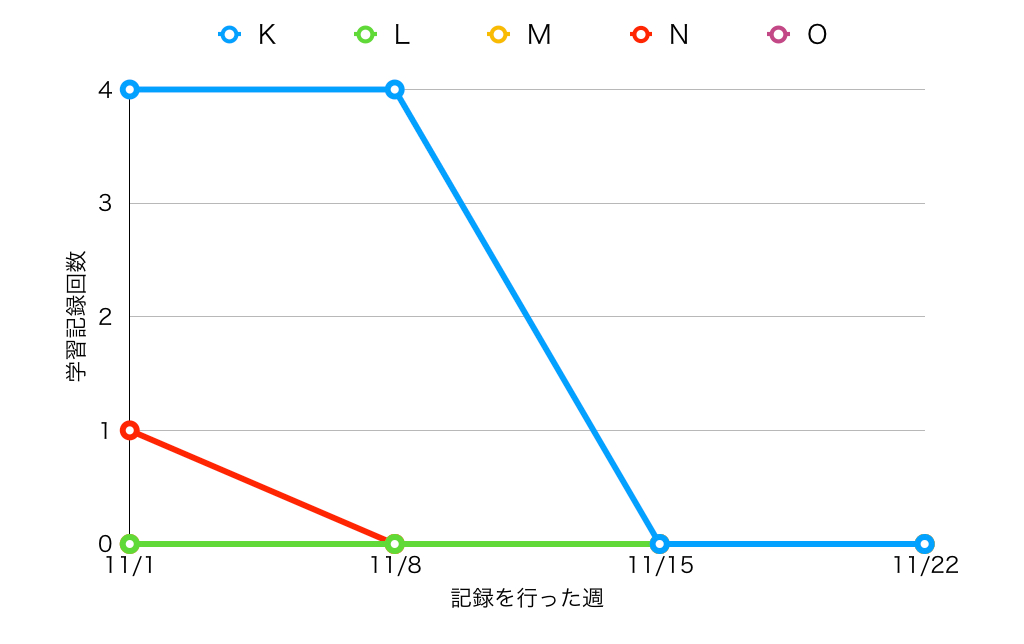
\includegraphics[width=10cm]{images/7/none_study_count.png}
  \caption{None群の学習記録回数の遷移}
  \label{fig:none_study_count}
  \end{center}
  \end{minipage}

\end{tabular}
\end{center}
\end{figure}

図~\ref{fig:same_app_open}, ~\ref{fig:wrong_app_open}, ~\ref{fig:none_app_open}に各群のアプリケーション起動回数の遷移を示す.
どの群においても,実験期間後半はアンケート回答のためにアプリを起動するのみであった.

\begin{figure}[htb]
\begin{center}
\begin{tabular}{c}

  \begin{minipage}[htb]{\linewidth}
  \begin{center}
  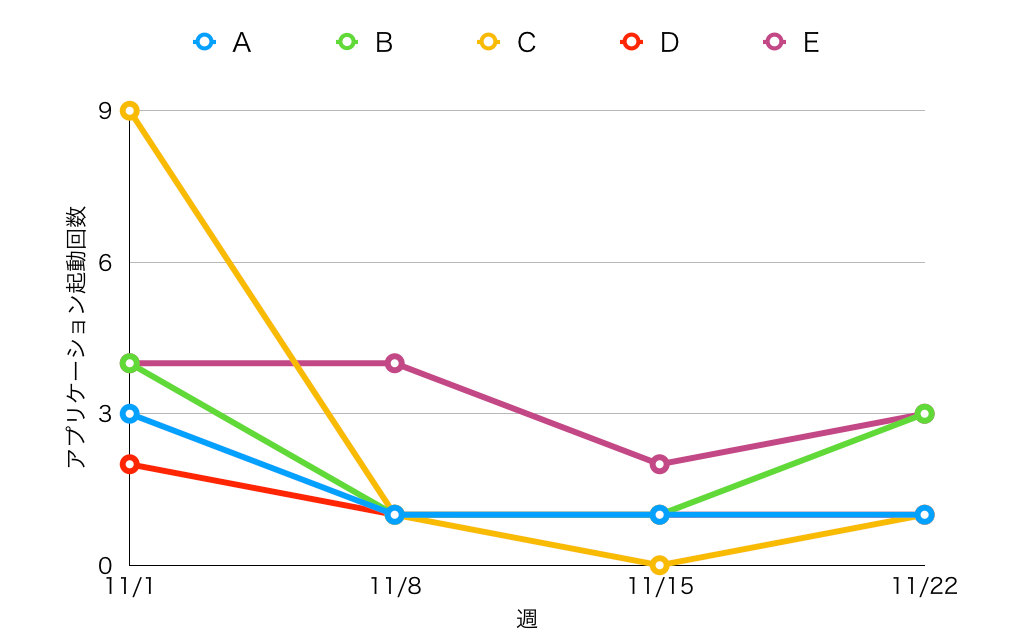
\includegraphics[width=10cm]{images/7/same_app_open.png}
  \caption{Same群のアプリケーション起動回数の遷移}
  \label{fig:same_app_open}
  \end{center}
  \end{minipage}

  \\

  \begin{minipage}[htb]{\linewidth}
  \begin{center}
  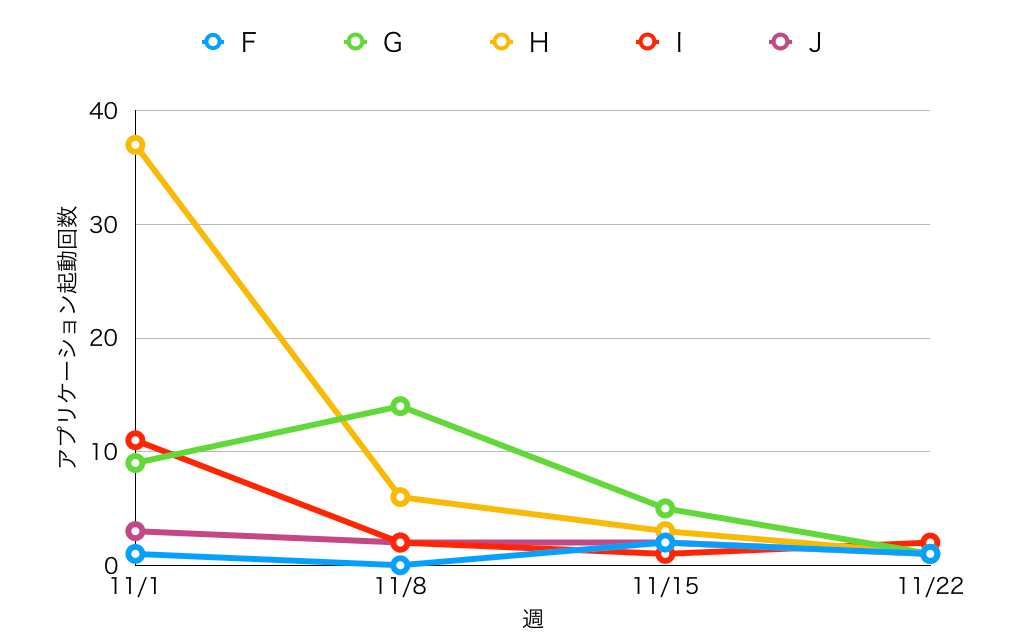
\includegraphics[width=10cm]{images/7/wrong_app_open.png}
  \caption{Wrong群のアプリケーション起動回数の遷移}
  \label{fig:wrong_app_open}
  \end{center}
  \end{minipage}

  \\

  \begin{minipage}[htb]{\linewidth}
  \begin{center}
  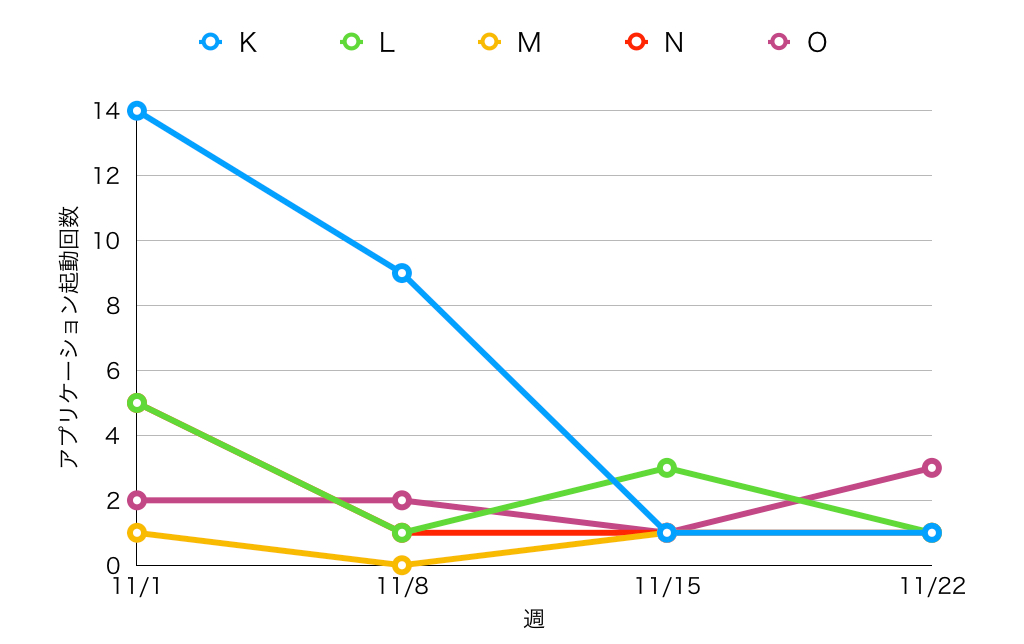
\includegraphics[width=10cm]{images/7/none_app_open.png}
  \caption{None群のアプリケーション起動回数の遷移}
  \label{fig:none_app_open}
  \end{center}
  \end{minipage}

\end{tabular}
\end{center}
\end{figure}

また,第1週目の動機づけタイプごとに被験者を分けた時の,一人あたりの平均総学習時間を図~\ref{fig:motivation_type_study_time}に,一人あたりの平均総学習記録回数を図~\ref{fig:motivation_type_study_count}に,一人あたりのアプリケーションの平均総起動回数を図~\ref{fig:motivation_type_app_open}に示す.
同一化的調整による動機づけを持った被験者らが学習時間,学習記録回数共に最も多く,次いで内的調整による動機づけを持った被験者らが多かった.取り入れ的調整による動機づけを持つ被験者らは全く学習を記録しなかった.

\begin{figure}[htb]
\begin{center}
\begin{tabular}{c}

\begin{minipage}[htb]{\linewidth}
  \begin{center}
  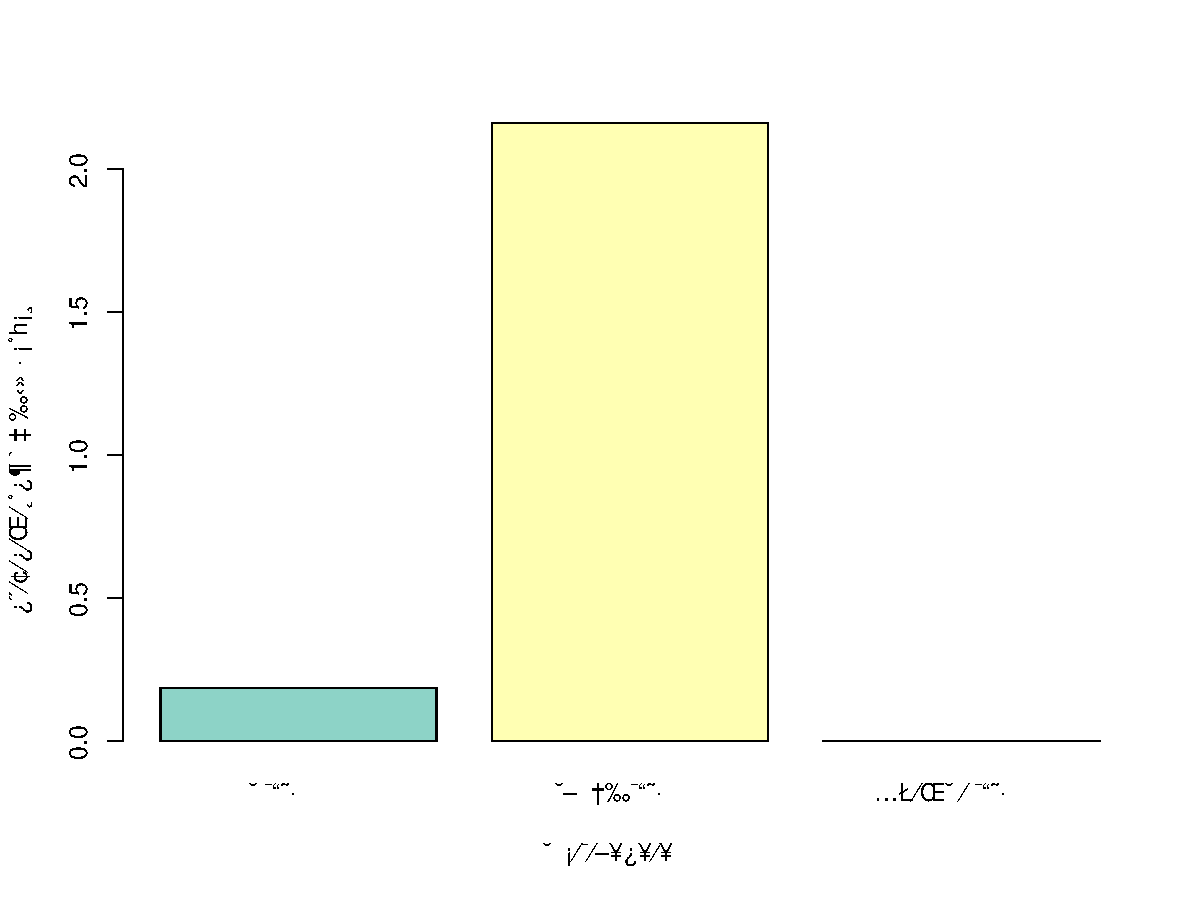
\includegraphics[width=9cm]{images/7/motivation_type_study_time.pdf}
  \caption{動機づけタイプ別の平均総学習時間}
  \label{fig:motivation_type_study_time}
  \end{center}
\end{minipage}

\\

\begin{minipage}[htb]{\linewidth}
  \begin{center}
  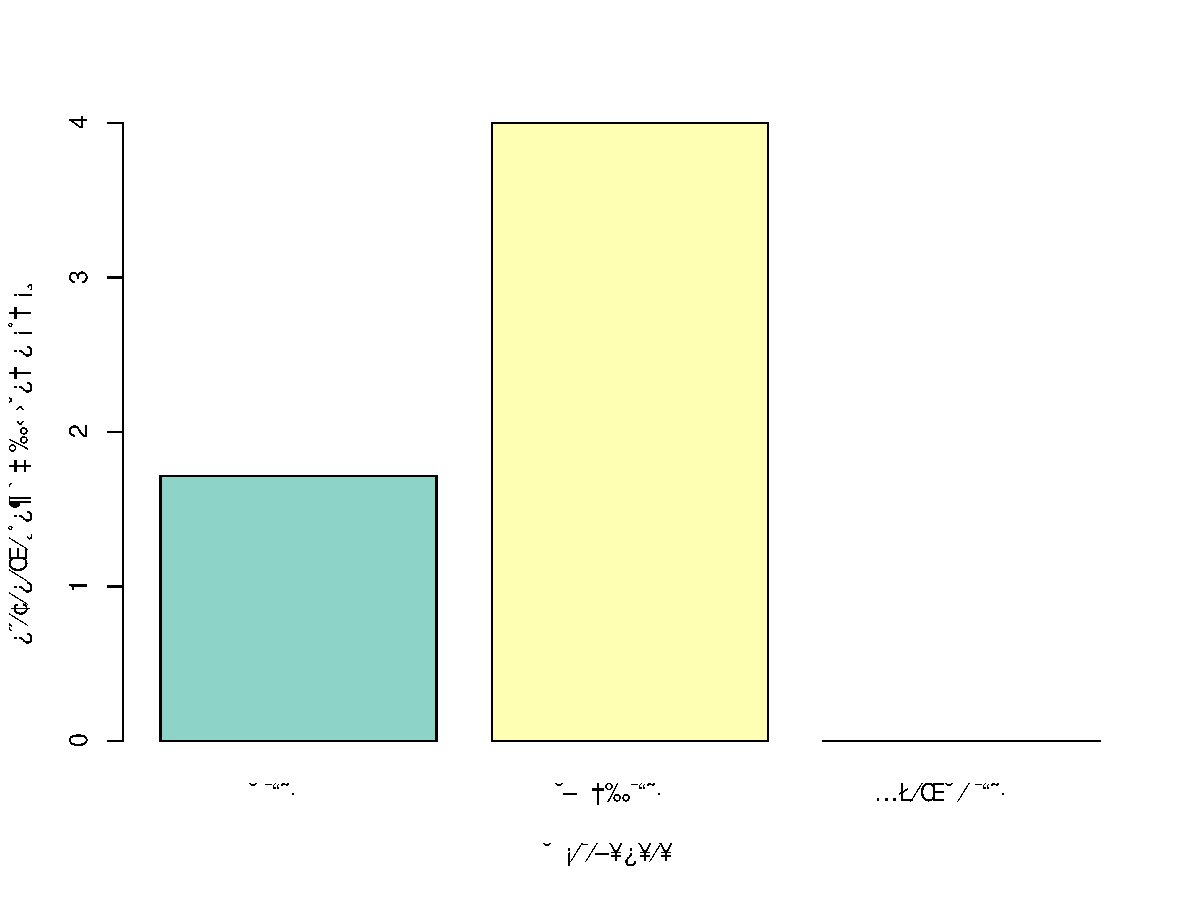
\includegraphics[width=9cm]{images/7/motivation_type_study_count.pdf}
  \caption{動機づけタイプ別の平均総学習記録回数}
  \label{fig:motivation_type_study_count}
  \end{center}
\end{minipage}

\\

\begin{minipage}[htb]{\linewidth}
  \begin{center}
  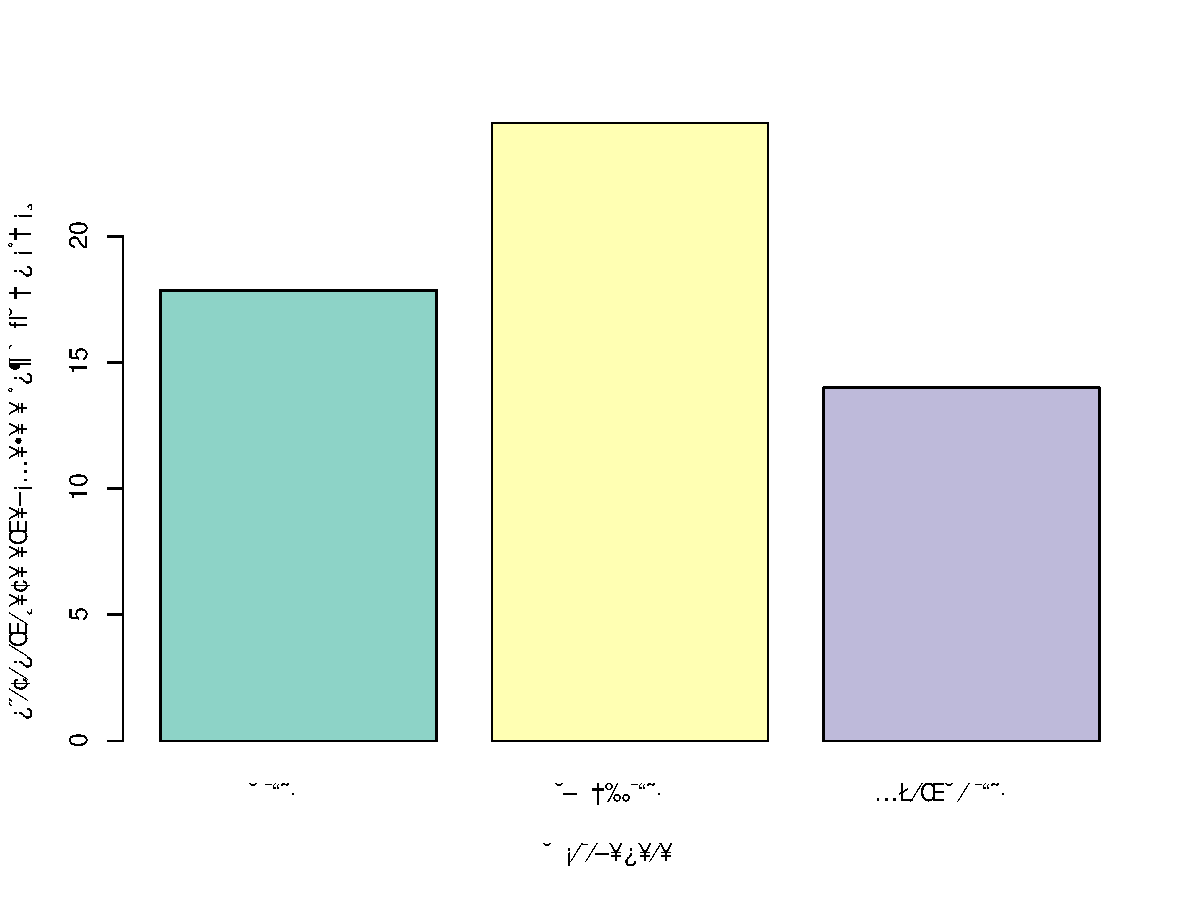
\includegraphics[width=9cm]{images/7/motivation_type_app_open.pdf}
  \caption{動機づけタイプ別のアプリケーション平均総起動回数}
  \label{fig:motivation_type_app_open}
  \end{center}
\end{minipage}

\end{tabular}
\end{center}
\end{figure}


\subsection{実験終了後アンケート}
実験終了後のアンケートにおいて,ポイント機能,ランキング機能,目標設定機能それぞれに対する評価を行ってもらった.
まずポイント機能に関して,``ポイント機能は言語学習に対するモチベーションを向上させたか"という設問に対しては,該当の機能が表示された被験者3名全員が``変わらなかった"と回答した.

続いてランキング機能について,``ランキング機能は言語学習に対するモチベーションを向上させたか"という設問に対して,該当の機能が表示された被験者6名全員が``変わらなかった"と回答した.
ランキング機能に対する自由記述において,``匿名ではモチベーションが上がらなかった"(被験者I)``誰も利用していないため興味がなかった"(被験者I)との回答を得た.

最後に目標設定機能について,``目標設定機能は言語学習に対するモチベーションを向上させたか"という設問に対して,該当の機能が表示された被験者5名中2名が``少し向上した"と回答し,残り3名は``変わらなかった"と回答した.

\section{考察}
本節では,評価実験で得られた様々な結果から考察を述べる.

\subsection{動機づけに対する影響}
本研究では,被験者の動機づけタイプに適したアプローチを行うことで,動機づけの向上及び内在化に効果があるかどうかを評価することを目的としている.
図~\ref{fig:same_study_count}, ~\ref{fig:wrong_study_count}, ~\ref{fig:none_study_count}からわかるように,どの群においても学習回数の増加は見られなかった.
実験期間の初めに学習を記録していた被験者は後半になるにつれアプリケーションを利用しなくなり,実験期間の初めに学習を記録していなかった被験者は実験期間中変わらずアプリケーションを利用しなかった.
一方で図~\ref{tb:same_motivation_type}, ~\ref{tb:wrong_motivation_type}, ~\ref{tb:none_motivation_type}の表からは動機づけタイプの明らかな変容は見られない.

図~\ref{fig:total_study_time}および~\ref{fig:total_study_count}から,Wrong群は学習時間が最も少ないものの学習記録回数は最も多い結果となった.
図~\ref{fig:wrong_records_ratio}からわかるように,Wrong群の学習記録はそのほとんどが実際に計測されて記録されたものである.
したがってWrong群の被験者らは,実際の学習活動に合わせてアプリケーションを利用しており,アプリケーション利用に対する動機づけが高いことが窺える.

図~\ref{tb:same_motivation_type}の表から,Same群の被験者Bは実験4週目に同一化的調整から取り入れ的調整に低下し,終了後は再度同一化的調整に戻っていることがわかる.
被験者Bは実験1週目と3週目のみで学習を記録しているが,アプリケーションを開いたのはアンケート回答時のみであったため,本システムによる動機づけの変容とは考えづらい.
同じくSame群の被験者Dは,実験3週目と4週目に同一化的調整から内的調整へと向上し,実験終了後は再度同一化的調整に戻った.
しかしながら被験者Dは実験期間を通して一度も学習を記録しておらず,アプリケーションを開いたのはアンケート回答時のみであったため,この動機づけの変容も本システムによる影響ではないと考えられる.

Wrong群の被験者Hは実験1週目に全被験者の中で最も多く学習を記録しており,その数9回である.
この時被験者Hに表示されていた機能は,同一化的調整に適した目標設定機能ではなくポイント機能であった.
図~\ref{tb:wrong_motivation_type}の表から,被験者Hは実験2週目に動機づけタイプが一度だけ内的調整に変容しており,これよりポイント機能が被験者Hの動機づけを内在化させた可能性が考えられる.
しかしながら2週目以降学習記録回数・アプリケーション起動回数共に低下し,3週目以降は一度も学習を記録しなかった.
したがって,ポイント機能が動機づけを内在化させた可能性はあるものの,その動機づけの持続性は低かったと考えられる.

同じくWrong群の被験者Gは,被験者の中で唯一学習記録回数が増加したユーザである.
被験者Gは1週目に1回であった学習記録回数を,2週目には9回に増加させた.
被験者Gの動機づけタイプは,実験期間中全ての週で内的調整と判定されており,実験1週目,2週目にはポイント機能が表示されていた.
したがって,ポイント機能が被験者Gの動機づけを向上させた可能性が考えられる.
一方で3週目以降は一度も記録を行わなかった.3週目にはランキング機能が表示されていた.
これより,ポイント機能によって向上された動機づけの持続性が低かったか,もしくはランキング機能が動機づけを低下させた可能性が示唆された.

None群においては,実験開始から終了までどの被験者にも動機づけタイプの変容は起こらなかった.

終了後のアンケートによれば,``(学習を)記録するメリットがない"(被験者I),``時間を記録・整理しても意味がないと考えている"(被験者J),``毎回記録するのが大変"(被験者C),``スマホを開くのが嫌だった"(被験者G)など,アプリケーション利用の動機づけが低い回答が多く見受けられた.

以上の結果から,本システムが被験者の学習に対する動機づけに与えた影響は少ないと言える.
一方で,被験者Gや被験者Hのように学習回数を向上させた被験者も存在する.
その要因として,彼らがアプリケーション利用に対して外的調整による動機づけを抱いていたために,ポイント機能の表示がアプリケーション利用回数の向上に影響を与えたのではないかと考えられる.
したがって,本システムはアプリケーション利用に対する動機づけに対して影響があり,それを向上させた可能性がある.
また,アプリケーションを用いて学習の動機づけを向上させようとする場合には,まず先にアプリケーション利用に対する動機づけを向上させる必要があることがわかった.

\subsection{動機づけ向上機能に対する評価}
実験終了後のアンケートより,ポイント機能及びランキング機能は学習に対する動機づけに対して影響を与えず,目標設定機能のみ学習に対する動機づけの向上に多少効果があった可能性がある.

ポイント機能に関して,被験者の中に報酬が要因となる外的調整による動機づけを抱く者がいなかったことから,動機づけの向上に影響を与えなかったと推測される.
また,このポイントが一切利益を持たないことから,報酬として捉えられなかった可能性も考えられる.

ランキング機能に関して,``匿名ではモチベーションが上がらなかった"(被験者I)という回答が得られたが,一方で``他者に自らの学習事情を知られたくない"(被験者J)との回答もあり,個人による差が見られた.
また,``誰も利用していないため興味がなかった"(被験者I)という回答があったように,このランキングは被験者全員を1つのグループとして生成したが,実験期間を通して活発に記録がされなかったことから,順位に変動のないランキングとなっていた.
これより,ランキングが学習に対する動機づけに影響を与えるためには,匿名でない友人間のランキングであること,もしくは活発な変動があることが条件として考えられる.

目標設定機能に関して,実装した3つの機能で唯一学習に対する動機づけが``少し向上した"という回答を得られた.
``少し向上した"とする回答者の中には内的調整を抱く被験者もおり,目標設定機能が同一化的調整だけでなく内的調整を抱くユーザに対しても有用である可能性が示された.

Wrong群は学習に対する動機づけの低下が起こることが予想されたが,実際には動機づけタイプに大きな変容は見られなかった(図~\ref{tb:wrong_motivation_type}の表).
この理由として,ポイント機能は実世界での利益を伴わないこと,ランキング機能は匿名でありほとんど機能しなかったことなどから,これらの機能が被験者に与える心理的影響が非常に小さかったと考えられる.

\subsection{動機づけタイプごとの考察}
どの被験者においても動機づけタイプの変容を確認できないことから,第1週目に判定された動機づけタイプを元に被験者をグループ分けし,考察を行う.
図~\ref{fig:motivation_type_study_time}, ~\ref{fig:motivation_type_study_count}, ~\ref{fig:motivation_type_app_open}からわかるように,同一化的調整による動機づけを持つ被験者が最も学習を記録した.
対して,取り入れ的調整による動機づけを持つ被験者は全く学習を記録せず,週に一度のアンケートに回答するのみであった.

同一化的調整とは目標のために学習を行なっている状態であり,要因の一部が外在的である.
学習に対する意欲がありつつ,一方で外的要素からの刺激も動機づけに影響を与えるため,本アプリケーションに興味を持ったのではないかと考えられる.

内的調整は好奇心から学習を行う状態で,要因が完全に内在化されているため,外的要素による影響を受けない.
したがって,本アプリケーションの利用に繋がらなかったと言える.

取り入れ的調整は競争のために学習を行う状態で,外的要因による影響が強い.
前項でも挙げたとおり本アプリケーションが提供する機能は心理的影響が小さかったこともあり,興味を抱かなかったのではないだろうか.

Same群,Wrong群,None群において動機づけの変容や学習記録状況に違いが見られないため,ポイント・ランキング・目標設定の3つの機能がそれぞれ異なる動機づけタイプに有用ということはなく,そもそも``学習記録アプリケーション"を提供すること自体が同一化的調整に対して有効なアプローチ手法である可能性が示唆された.

\section{まとめ}
本章では,Stuguinシステムで得られたデータから動機づけの向上を評価し,考察について述べた.
次章では,本研究における今後の展望と本論文のまとめを述べる.
